\documentclass[a4paper, 12pt]{article}
\usepackage{amsmath}
\usepackage{color}
\usepackage{dsfont}
\usepackage[utf8]{inputenc}
\usepackage{graphicx}
\usepackage[left=2cm, right=2cm, bottom=3cm, top=2cm]{geometry}
\usepackage{natbib}
\usepackage{microtype}


\definecolor{orange}{rgb}{1, 0.5, 0}
\definecolor{green}{rgb}{0, 0.5, 0}

\newcommand{\hypers}{\boldsymbol{\alpha}}
\newcommand{\params}{\boldsymbol{\theta}}
\newcommand{\data}{\boldsymbol{x}}
\newcommand{\info}{\boldsymbol{M}}
\newcommand{\x}{x}
\newcommand{\todo}{\color{orange} \bf}


\title{Crystals}
\author{Brendon J. Brewer}
\date{}

\begin{document}
\maketitle

%\abstract{\noindent Abstract}

% Need this after the abstract
\setlength{\parindent}{0pt}
\setlength{\parskip}{8pt}

\section{The prior information}



\subsection{The shape of the model curve}
The algorithm fits the data with a model curve
$f(\x)$, defined between $\x=\x_{\rm min}$ and $\x=\x_{\rm max}$,
which is assumed to be a sum of the following components:
\begin{enumerate}
\item A background component
\item $N_{\rm wide}$ wide gaussians
\item $N_{\rm narrow}$ narrow gaussians, to model the spikes.
\end{enumerate}

We compute the posterior distribution for the unknown parameters of the
components, and use \citep{dnest4} to generate samples from that posterior
distribution, representing plausible parameter values. From each sample,
it is possible to compute the crystallinity, making it straightforward to
calculate the marginal posterior distribution of the crystallinity, describing
uncertainty about its value in the light of the data.


The background component is assumed to be piecewise linear
{\todo between $\x=x_{\rm min}$ and $\x=10$, between $\x=10$ and $\x=40$,
and between $\x=40$ and $\x=\x_{\rm max}$}.
We parameterise the background component using
five parameters. Firstly, there is a mean level $b$, which sets the
typical amplitude of the background component. There are also four parameters
$n_1, ..., n_4$, which set the positions of four control points:
\begin{align}
\left(\x_{\rm min}, be^{n_1}\right) \nonumber\\
\left(10, be^{n_2}\right) \nonumber\\
\left(40, be^{n_3}\right) \nonumber\\
\left(\x_{\rm max}, be^{n_4}\right) \nonumber
\end{align}
The value of the background component at any other point is found by
linear interpolation. Figure~\ref{fig:background} shows three example
background curves generated from this parameterisation, with typical
values of the parameters.

\begin{figure}
\centering
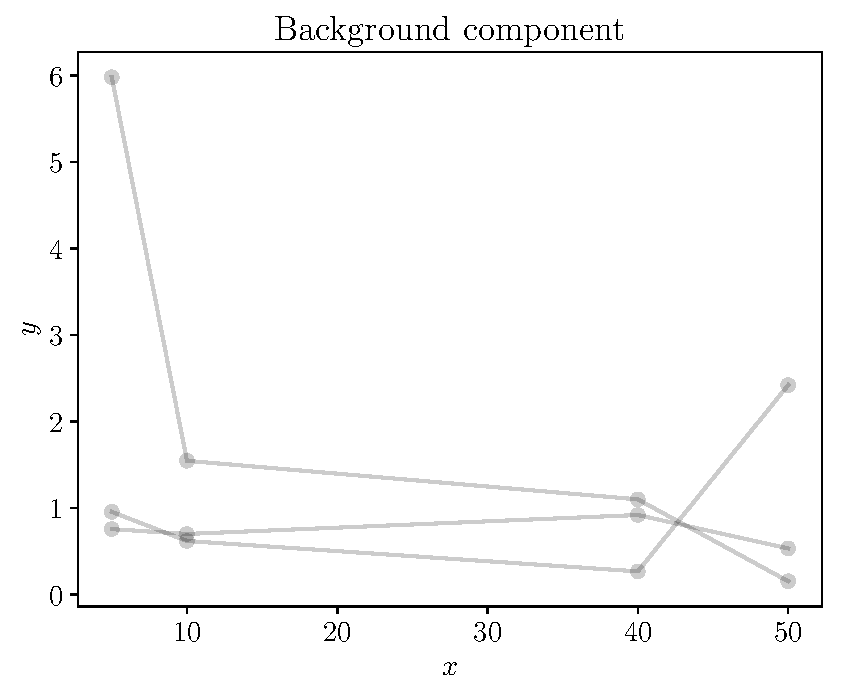
\includegraphics[width=0.7\textwidth]{figures/background.pdf}
\caption{\label{fig:background}}
\end{figure}



\subsection{Prior probability distributions}

The joint prior distribution for the hyperparameters, parameters, and data,
is written $p(\hypers, \params, \data | \info)$, and is usually factorised
in this way:
\begin{align}
p(\hypers, \params, \data | \info) &=
    p(\hypers | \info)p(\params | \hypers, \info)
    p(\data | \params, \hypers, \info)\\
    &= p(\hypers | \info)p(\params | \hypers, \info)
    p(\data | \params, \info)
\end{align}
where the first step is true in general by the product rule, and the second
step assumes that knowing the parameters would make the hyperparameters
irrelevant when predicting what data would be observed.

All of the assumptions are given in Table~\ref{tab:priors}.

\begin{table}
\centering
\begin{tabular}{|lll|}
\hline
{\bf Quantity}      &   {\bf Meaning}   &  {\bf Prior distribution}\\
\hline
{\em Hyperparameters} & &\\
$N_{\rm narrow}$   &   Number of narrow spikes    &  $\propto 1/(N_{\rm narrow}+1)$, $N_{\rm narrow} \in \{0, 1, ..., 300\}$ \\
$N_{\rm wide}$   &   Number of wide spikes    &  $\propto 1/(N_{\rm wide}+1)$,
$N_{\rm wide} \in \{0, 1, ..., 300\}$ \\

\hline
{\em Parameters}& &\\
$\sigma_0$ &    Constant noise level  &   $\ln(\sigma_0) \sim \textnormal{Laplace}(0,5)$\\
$\sigma_1$ &    Noise proportionality   &  $\ln(\sigma_1) \sim \textnormal{Laplace}(0,5)$ \\
$\nu$     &   Shape parameter for residuals   &   LogUniform$(1, 1000)$\\
$b$       & Mean background level       & Laplace$(0, 5)$\\
$\{n_1, ..., n_4\}$  & Background deviations & iid Normal$(0,1)$\\
\hline
{\em Data}&&\\
\hline
$\{y_1, y_2, ..., y_n\}$  &   Measurements    & Student $t(f(x_i; \params), ,\nu)$\\
\hline
{\em Prior information}&&\\
\hline
$n$ & Number of measurements & given\\
$\{x_1, x_2, ..., x_n\}$  & $x$-values of measurements & given \\
\hline
\end{tabular}
\caption{\label{tab:priors}}
\end{table}

The Laplace, or biexponential, distribution with location parameter $a$ and
scale parameter $b$ has probability density
\begin{align}
p(x | a, b) &= \frac{1}{2b}\exp\left[-\frac{|x - a|}{b}\right].
\end{align}


The shape of the model function $f(x)$ is therefore
\begin{align}
f(x) &= f_{\rm bg}(x) + f_{\rm wide}(x) + f_{\rm narrow}(x)
\end{align}
and the crystallinity is
\begin{align}
C &= \frac{\int f_{\rm wide}(x) \, dx}
          {\int f_{\rm wide}(x) \, dx + \int f_{\rm narrow}(x) \, dx}
\end{align}


\bibliographystyle{plainnat}
\bibliography{references}

\end{document}

